\addcontentsline{toc}{chapter}{345 - Matrix Sum}
\chapter*{345 - Matrix Sum}

\index{Hungarian algorithm}
We define the Matrix Sum of a matrix as the maximum sum of matrix elements with each element being the only one in his row and column. For example, the Matrix Sum of the matrix below equals 3315 ( = 863 + 383 + 343 + 959 + 767):

\begin{figure}[H]
    \centering
    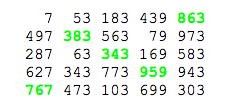
\includegraphics[scale=0.5]{images/pe345a.png}
    \caption{Caption}
    \label{fig:pe345a}
\end{figure}


Find the Matrix Sum of:

\begin{figure}[H]
    \centering
    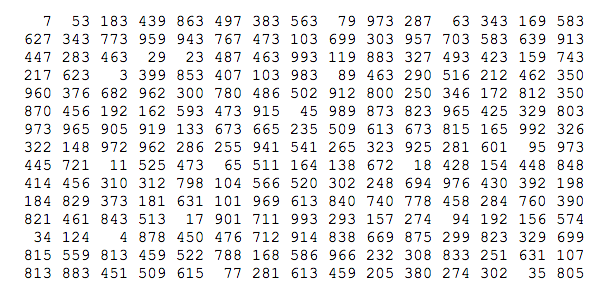
\includegraphics[scale=0.5]{images/pe345b.png}
    \caption{Caption}
    \label{fig:pe345b}
\end{figure}


\section*{Solution}

This problem can be seen as a Minimum Bipartite Matching Problem. From one side we have the rows, and in the other side we have the columns, and we must find the minimum 1-1 matching. In other words, for each row we must assign only one column, and the sum of all matches must be minimum.\\

For this problem we can use \textit{Hungarian Algorithm}, which if my memory is correct runs in $O(n^4)$, where $n$ is the size of the matrix. In \cite{hungarian} there is a great explanation of the algorithm.

